\documentclass[a4paper,12pt]{article}
\usepackage[english,russian]{babel}
\usepackage[utf8]{inputenc}
\usepackage{latexsym,mathrsfs}
\usepackage{stmaryrd, enumitem}
\usepackage{amsthm,amsfonts,amssymb,amsmath}
\usepackage{geometry}
\usepackage{tempora}
\usepackage{graphicx}
\usepackage{url}
\usepackage{listingsutf8}


\geometry{top=17mm}  \geometry{bottom=20mm}
\geometry{left=17mm} \geometry{right=17mm}
\linespread{1.1}
\parindent=5mm

\def\titleK#1{\begin{center}{\Large\textbf{#1}}\end{center}}
\def\authorK#1{\begin{center}{#1}\end{center}}

\newenvironment{abstractK}{}

\newtheorem{theorem}{Теорема}
\newtheorem{lemma}{Лемма}
\newtheorem{corollary}{Следствие}
\newtheorem{proposition}{Предложение}
\newtheorem{statement}{Утверждение}
\theoremstyle{definition}
\newtheorem{definition}{Определение}
\newtheorem{problem}{Задача}
\newtheorem{question}{Вопрос}
\newtheorem{conjecture}{Гипотеза}
\newtheorem{construction}{Конструкция}
\newtheorem{remark}{Замечание}

%ВАЖНО: Просьба пользоваться имеющимися окражениями-теоремами
%ВАЖНО: Не менять и не добавлять ничего выше этой строки.
%Изменения вносить только внутри окружения \begin{document}\end{document}

\begin{document}

%Название доклада
\titleK{Исследование аппаратно-программных реализаций алгоритмов защиты информации}

%Информация об авторах (ЗАМЕНИТЕ на свои данные)
\authorK{Д.~С.~Соловьёв$^{1}$, А. Р. Труфанов$^{2}$, С. В. Копылова$^{2}$, Д. А. Бондаренко$^{2}$,  А. С. Марков$^{2}$, 
\\В. М. Завьялова$^{3}$, Э. А. Салеев$^{4}$, А. В. Тюндин$^{5}$
\\$^{1}$Южный федеральный университет 
\\$^{2}$НИЯУ МИФИ
\\$^{3}$СПГУ
\\$^{4}$Казанский (Приволжский) федеральный университет
\\$^{5}$НГТУ им. Р. Е. Алексеева
\\{\bf E-mail:} dsolove@sfedu.ru, tar003@campus.mephi.ru,  SonyCop26@yandex.ru, bondarenk0dennis@yandex.ru, senya1107@mail.ru, varvara.zavyalova.007@ya.ru,  emilic\_saleeve@mail.ru, AlexanderTyundin@yandex.ru}

\begin{abstract}
{\bf Актуальность:} Проект направлен на изучение методов реализаций широко распространенных алгоритмов криптографической защиты информации; изучение алгоритмов защиты от статического и динамического анализа, а также на развитие у исследователя нестандартного подхода к анализу надежности механизмов защиты.
\\
{\bf Ключевые слова:} \textit{проверка надежности системы защиты исполняемого кода, статический и динамический анализ, информационная безопасность.} 
\end{abstract}

\begin{abstractK}

\section*{Введение}

В условиях стремительного развития информационных технологий и повсеместной цифровизации всё больше критически важных функций реализуется в программном обеспечении. Это делает программные продукты привлекательной целью для злоумышленников, стремящихся получить несанкционированный доступ к алгоритмам и бизнес-логике приложения. Конкретные программные реализации алгоритмов, в настоящее время, все чаще составляют коммерческую тайну. Таким образом, конкретная реализация программного продукта также является данными, утрата которых может нанести чувствительный финансовый и репутационный ущерб коммерческой компании.

Наиболее действенными инструментами в арсенале нарушителей при исследовании программного продукта остаются методы статического и динамического анализа, позволяющие восстановить чувствительные элементы логики приложения и бизнес-процесса.

Современные средства анализа – от дизассемблеров и отладчиков до систем автоматизированного анализа программной реализации становятся всё более доступными и мощными. Это значительно снижает порог входа для злоумышленников и делает традиционные подходы к защите, такие как простая обфускация или упаковка исполняемых файлов, недостаточно эффективными. Настоящая работа представляет обзор и оценку применимости широко распространенных методов зашщиты исполняемого кода.

\section*{Цель исследования:}
Целью исследования является анализ и сравнительная оценка эффективности современных методов защиты исполняемого кода от статического и динамического анализа, а также исследование алгоритмов обнаружения криптографических примитивов в программных реализациях для выработки рекомендаций по повышению надежности систем защиты.

\section*{Задачи исследования:}
\begin{enumerate}
    \item Обзор современных алгоритмов защиты от статического и динамического анализа;
    \item Исследование конкретной реализации алгоритмов защиты от статического и динамического анализа;
    \item Исследование алгоритмов поиска реализаций широко распространённых методов криптографической защиты информации;
\end{enumerate}

\section*{Объект исследования}

Объектом исследования является исполняемый файл, используемый в операционных системах семейства Windows и применяющий 64-битную архитектуру, реализующий механизмы защиты программного кода и взаимодействующий с аппаратным средством безопасности. В соответствии с целью было проведено исследование. По внешним признакам используемый программно-аппаратный комплекс напоминает решения класса Рутокен, который сертифицирован по четвёртому уровню доверия по линии ФСТЭК и подтверждает высокий уровень безопасности при работе с конфиденциальной информацией. Приложение обращается к специализированному интерфейсу работы с защищённым носителем, а ключевой материал не наблюдается в пользовательском модуле в открытом виде.


\section*{1. Обзор современных алгоритмов защиты от статического и динамического анализа}

В соответствии с задачами исследования содержательная часть работы строится как обзор основных групп защитных механизмов, применяемых для противодействия статическому и динамическому анализу исполняемого кода. К современным средствам защиты исполняемого кода относятся антиотладочные ловушки, самоотладка и шифрование кода.

\subsubsection*{1.1. Техника Trap-Based (антиотладка на основе исключений)}

Среди множества антиотладочных техник особое место занимает группа методов, основанных на использовании аппаратных и программных \textit{исключительных ситуаций} (traps). Эти методы, обозначаемые в литературе как \textit{Trap-Based anti-debugging} (далее ``Trap-Based'') \cite{trapbased}, эксплуатируют фундаментальное различие в обработке исключительных ситуаций между обычным исполнением и исполнением под управлением отладчика. Дополнительное измерение данной проблематики связано с использованием привилегированных инструкций --- команд процессора, выполнение которых в пользовательском режиме (Ring~3) штатно приводит к генерации исключений, перехватываемых ядром операционной системы.

\subsubsection*{1.1.1. Формальная модель}

Механизм обработки исключений (exceptions) является центральным для реализации техники Trap-Based. Исключения могут быть вызваны как аппаратно (например, при обращении к недействительной памяти), так и программно --- путём выполнения специальных инструкций.

Ключевое различие, на котором строятся Trap-Based методы, заключается в следующем:

\begin{itemize}
    \item \textbf{В отсутствие отладчика} исключение передаётся на обработку зарегистрированному обработчику исключений операционной системы или пользовательскому обработчику, установленному приложением.
    \item \textbf{При наличии подключённого отладчика} исключение перехватывается отладчиком до того, как оно достигнет обработчика приложения.
\end{itemize}

Это поведение является следствием архитектуры отладочных интерфейсов: отладчик регистрируется в системе как обработчик отладочных событий (debug events) для отлаживаемого процесса. Любое исключение, возникающее в процессе, сначала передаётся отладчику, который может его обработать, проигнорировать или передать дальше.

Введём формальное описание поведения системы. Пусть:

\begin{itemize}
    \item $P$ --- защищаемое приложение;
    \item $D$ --- отладчик;
    \item $E$ --- множество исключений, генерируемых процессором;
    \item $H_P$ --- обработчик исключений, установленный приложением;
    \item $H_{OS}$ --- обработчик исключений операционной системы.
\end{itemize}

Тогда для некоторой инструкции $I \in \mathcal{I}$, генерирующей исключение $e \in E$:

\[
\text{flow}(I,e)=
\begin{cases}
H_P(e), & \text{если } D \text{ не подключён};\\
D(e), & \text{если } D \text{ подключён и перехватывает } e;\\
H_{OS}(e), & \text{если } D \text{ подключён, но передаёт } e \text{ системным обработчикам}.
\end{cases}
\]

Техника ``Trap-Based'' основана на измерении различия в потоке управления: приложение выполняет инструкцию, генерирующую исключение, и проверяет, был ли вызван его собственный обработчик. Если обработчик не был вызван, делается вывод о присутствии отладчика.

\subsubsection*{1.1.2. Классификация методов}

Методы ``Trap-Based'' могут быть классифицированы по типу используемого исключения и способу его генерации.

\paragraph{Использование программных точек останова}

Рассматриваемые методы используют технику установки программных точек останова при выполнении приложения. Примером применения такой техники может быть выполнение инструкции \texttt{INT3} (однобайтовый опкод \texttt{0xCC}). При выполнении \texttt{INT3} процессор генерирует исключение \texttt{EXCEPTION\_BREAKPOINT} (0x80000003 в Windows) или сигнал \texttt{SIGTRAP} в Unix-подобных системах.

Альтернативой прямому использованию \texttt{INT3} может быть применение функций \texttt{DebugBreak} (Windows) и \texttt{raise(SIGTRAP)} (POSIX). Их использование обеспечивает переносимость на уровне API \cite{intel80386}.

При применении рассматриваемого метода приложение устанавливает собственный обработчик исключений (например, используя функцию \texttt{SetUnhandledExceptionFilter} в Windows или \texttt{signal(SIGTRAP, handler)} в Linux) и выполняет инструкцию, связанную с программной точкой останова. В результате:

\begin{itemize}
    \item Без отладчика: исключение достигает обработчика приложения $\rightarrow$ обработчик выполняется $\rightarrow$ приложение продолжает работу.
    \item С отладчиком: отладчик перехватывает исключение $\rightarrow$ обработчик приложения не вызывается $\rightarrow$ приложение детектирует отладку.
\end{itemize}

\paragraph{Использование Trap Flag (TF)}

Аналогичный эффект можно получить, устанавливая флаг пошагового выполнения (TF) \cite{intel80386}. Флаг Trap Flag (TF) --- это бит №8 регистра \texttt{EFLAGS} (или \texttt{RFLAGS} в x86-64). Когда этот флаг установлен в~1, процессор генерирует исключение \texttt{EXCEPTION\_SINGLE\_STEP} (0x80000004) после выполнения каждой инструкции. Именно этот механизм используется отладчиками для реализации пошагового исполнения (single-stepping).

Приложение устанавливает обработчик исключений, затем программно устанавливает флаг TF (например, через инструкции \texttt{PUSHF}/\texttt{POPF} или посредством операции \texttt{OR} над регистром флагов). В результате поведение приложения меняется следующим образом:

\begin{itemize}
    \item Без отладчика: после каждой инструкции генерируется исключение $\rightarrow$ вызывается обработчик приложения $\rightarrow$ обработчик может сбросить TF и продолжить исполнение.
    \item С отладчиком: отладчик, как правило, перехватывает исключения single-step и сбрасывает TF. Обработчик приложения не вызывается $\rightarrow$ детектирование отладки.
\end{itemize}

\paragraph{Привилегированные инструкции ввода-вывода как механизм Trap-Based}

Особый интерес в контексте методов Trap-Based представляют привилегированные инструкции ввода-вывода, такие как \texttt{IN}, \texttt{INS}, \texttt{OUT}, \texttt{OUTS}. Согласно \cite{intel80386}, эти инструкции предназначены для прямого доступа к портам ввода-вывода устройства и, в силу архитектурных ограничений, не могут быть выполнены произвольным пользовательским приложением без соответствующих разрешений.

\paragraph{Архитектурные основы: IOPL и карта разрешений ввода-вывода}

Согласно \cite{intel80386}, в защищённом режиме процессор использует два механизма для контроля доступа к операциям ввода-вывода:

\begin{enumerate}
    \item \textbf{Поле IOPL (I/O Privilege Level)} в регистре \texttt{EFLAGS} определяет минимальный уровень привилегий (CPL), необходимый для выполнения инструкций ввода-вывода. Инструкции \texttt{IN}, \texttt{INS}, \texttt{OUT}, \texttt{OUTS}, а также \texttt{CLI} и \texttt{STI} могут быть выполнены только при условии \texttt{CPL <= IOPL}. В большинстве современных операционных систем (Windows, Linux, macOS) значение IOPL устанавливается равным~0, что делает выполнение этих инструкций из пользовательского режима (Ring~3, CPL~=~3) невозможным.
    \item \textbf{Карта разрешений ввода-вывода (I/O Permission Bitmap)} в сегменте состояния задачи (TSS) обеспечивает более тонкую гранулярность контроля доступа к отдельным портам. Даже если \texttt{CPL > IOPL}, процессор обращается к этой карте; если соответствующий бит равен~0, операция разрешается, иначе генерируется исключение общей защиты (\#GP).
\end{enumerate}

\paragraph{Механизм генерации исключений}

При попытке выполнения инструкции \texttt{IN} или \texttt{OUT} из кода, выполняющегося на уровне привилегий Ring~3, возможны следующие сценарии:

\begin{itemize}
    \item Если \texttt{CPL > IOPL}, процессор генерирует исключение общей защиты (\#GP).
    \item В Windows NT и последующих версиях это исключение перехватывается ядром, которое, как правило, завершает процесс, сгенерировав исключение \texttt{EXCEPTION\_PRIV\_INSTRUCTION} (0xC0000096).
    \item В некоторых конфигурациях (например, при работе в режиме Virtual~8086 или при наличии специальных драйверов) исключение может быть обработано иначе, однако для штатного пользовательского приложения выполнение инструкций \texttt{IN}/\texttt{OUT} гарантированно приводит к исключению.
\end{itemize}

Именно это свойство --- гарантированная генерация исключения при выполнении привилегированной инструкции из Ring~3 --- делает эффективным применение инструкций \texttt{IN} и \texttt{OUT} для реализации методов Trap-Based.

Принцип реализации идентичен классическим Trap-Based методам:

\begin{enumerate}
    \item Приложение регистрирует собственный обработчик исключений (SEH, VEH в Windows или сигнальный обработчик в Linux).
    \item Приложение выполняет привилегированную инструкцию, например \texttt{IN AL, DX} или \texttt{OUT DX, AL}.
    \item В отсутствие отладчика процессор генерирует исключение \#GP, которое доставляется операционной системе; ОС транслирует его в структурированное исключение и передаёт зарегистрированному обработчику приложения. Обработчик перехватывает исключение, корректирует поток выполнения (например, пропуская инструкцию посредством увеличения значения \texttt{EIP}) и продолжает работу.
    \item При наличии отладчика исключение перехватывается до того, как оно достигнет обработчика приложения. Если отладчик не настроен на передачу данного исключения приложению, обработчик приложения не вызывается, что позволяет приложению обнаружить факт отладки.
\end{enumerate}

\subsubsection*{1.1.3. Выводы}

\paragraph{Преимущества}

\begin{itemize}
    \item \textbf{Высокая надёжность.} Выполнение привилегированных инструкций в Ring~3 является архитектурно запрещённым действием. Исключение \#GP генерируется непосредственно процессором \cite{intel80386} и не может быть обработано на уровне приложения без участия ядра.
    \item \textbf{Сложность обхода.} Для сокрытия своего присутствия отладчик должен корректно эмулировать выполнение привилегированной инструкции либо передавать исключение приложению, что требует дополнительной реализации.
\end{itemize}

\paragraph{Особенности применения}

\begin{itemize}
    \item \textbf{Зависимость от платформы.} Поведение строго определено для архитектуры x86/x64; на других архитектурах (ARM, RISC-V) механизмы могут отличаться.
    \item \textbf{Потенциальная нестабильность.} В некоторых виртуализированных средах (например, при использовании Hyper-V) выполнение привилегированных инструкций может сопровождаться побочными эффектами.
    \item \textbf{Сигнатура в коде.} Наличие привилегированных инструкций легко выявляется средствами статического анализа.
    \item \textbf{Особенности Windows.} При отсутствии обработчика исключений выполнение привилегированной инструкции может привести к генерации исключения \texttt{EXCEPTION\_PRIV\_INSTRUCTION} и завершению процесса.
\end{itemize}


\subsubsection*{1.2. Self-Debug (самоотладка)}

Техника \textit{Self-Debugging} основана на использовании штатного отладочного интерфейса операционной системы не исследователем, а самим механизмом защиты. Защищаемое приложение создаёт вспомогательный процесс, поток или сервисный компонент, который подключается к нему как отладчик и получает отладочные события. В результате отладочный ресурс процесса оказывается занят, а последующее подключение внешнего отладчика либо завершается ошибкой, либо приводит к наблюдаемому изменению порядка доставки событий \cite{selfdebugging,windowsinternals}.

В обзорном смысле самоотладка занимает промежуточное положение между проверками среды выполнения и ловушками на исключениях: она не скрывает код сама по себе, но меняет доступность динамического наблюдения. Поэтому к данному классу удобно относить как собственно монополизацию отладочного интерфейса, так и вспомогательные проверки системных признаков отладки, включая обращения к структуре
\[
\underbrace{\texttt{P}\quad\texttt{E}\quad\texttt{B}}_{\text{Process Environment Block: BeingDebugged, NtGlobalFlag, параметры процесса}}.
\]
Такая запись подчёркивает, что \texttt{PEB}-проверки являются не самостоятельной целью защиты, а источником наблюдаемых признаков для антиотладочной логики.

\subsubsection*{1.2.1. Формальная модель}

Пусть $P$ --- защищаемый процесс, $G$ --- процесс-защитник, выполняющий роль внутреннего отладчика, а $D$ --- внешний отладчик исследователя. Для современных ОС характерно ограничение, при котором активная отладочная привязка процесса единственна. Тогда состояние отладочного интерфейса можно представить как частичную функцию
\[
\operatorname{dbg}(P) \in \{\varnothing, G, D\}.
\]
Если защита первой переводит систему в состояние $\operatorname{dbg}(P)=G$, попытка установить $\operatorname{dbg}(P)=D$ нарушает инвариант единственности отладчика. Защитный код может использовать сам факт отказа системного вызова, изменение статуса отладочного порта или отсутствие ожидаемого события как индикатор вмешательства.

Для признаковых проверок, сопровождающих самоотладку, пусть $S=\{s_1,\ldots,s_n\}$ --- множество наблюдаемых признаков среды выполнения, а $f_i(P)$ --- функция извлечения $i$-го признака из состояния процесса или ОС. Тогда антиотладочная проверка может быть представлена предикатом
\[
A(P)=\bigvee_{i=1}^{n} \left(f_i(P) \in V_i\right),
\]
где $V_i$ --- множество значений, интерпретируемых как характерные для исполнения под отладчиком. При истинности $A(P)$ приложение может завершиться, перейти к ложной ветви, исказить результат вычислений, отложить расшифрование кода или активировать дополнительные проверки.

\subsubsection*{1.2.2. Классификация методов}

Методы самоотладки и связанные с ними проверки можно классифицировать по используемому системному ресурсу и по способу реакции на вмешательство.

\paragraph{Монополизация отладочного интерфейса}

Типовая схема включает запуск защищаемого процесса в режиме, допускающем подключение вспомогательного компонента, подключение внутреннего отладчика к целевому процессу, переход к циклу обработки отладочных событий и контроль целостности связки ``защищаемый процесс --- процесс-защитник''. Если внешний исследователь пытается подключить отладчик, операция завершается ошибкой либо меняет порядок доставки событий.

\paragraph{Диспетчеризация исключений внутренним отладчиком}

Поскольку защитный компонент получает исключения раньше пользовательского обработчика, он может использоваться как диспетчер защищённого потока управления: передавать приложению только допустимые исключения, скрывать служебные ловушки, восстанавливать контекст после выполнения проверок и синхронизировать расшифрование отдельных участков кода. Поэтому самоотладка естественно сочетается с Trap-Based-подходом.

\paragraph{Проверки PEB и системных признаков}

Для Windows характерны проверки поля \texttt{BeingDebugged} в структуре \texttt{PEB}, флага \texttt{NtGlobalFlag}, результатов функций \texttt{IsDebuggerPresent} и \texttt{CheckRemoteDebuggerPresent}, а также низкоуровневых запросов \texttt{NtQueryInformationProcess} к состоянию отладочного порта, объекта отладки и флагов процесса \cite{windowsinternals,msdebugapi}. Прямые обращения к \texttt{PEB} могут скрываться арифметической обфускацией адресов, косвенными вызовами, виртуальными таблицами и рассеиванием проверок по графу управления.

\subsubsection*{1.2.3. Выводы}

Самоотладка повышает стоимость динамического анализа за счёт занятия отладочного интерфейса и контроля доставки событий, однако не препятствует статическому восстановлению кода. Её ограничения связаны с зависимостью от ОС, прав процесса и наблюдаемостью вспомогательных компонентов: исследователь может попытаться завершить процесс-защитник, подменить параметры отладочного порта, запустить приложение в подготовленной среде или эмулировать ответы системного API. Поэтому самоотладка обычно применяется совместно с Trap-Based-проверками, контролем окружения и шифрованием кода.

\subsubsection*{1.3. Code Cipher (шифрование кода)}

Методы шифрования кода направлены на разрыв связи между статическим представлением исполняемого файла и фактически выполняемой логикой. В отличие от синтаксической обфускации, меняющей форму уже доступного кода, \textit{Code Cipher} предполагает, что существенная часть программы хранится в преобразованном виде и становится исполняемой только в заданный момент времени. Классические таксономии обфускации рассматривают такие преобразования как часть более общей задачи усложнения понимания программы при сохранении её наблюдаемой функциональности \cite{collberg,obfuscation}.

\subsubsection*{1.3.1. Формальная модель}

Пусть $C$ --- защищаемый фрагмент программы, $T_k$ --- обратимое преобразование с параметром $k$, а $C'=T_k(C)$ --- представление фрагмента в исполняемом файле. Во время выполнения защитный механизм проверяет набор условий $Q$ и, если они выполнены, восстанавливает код:
\[
C = T_k^{-1}(C'), \quad \text{если } Q(P,E)=1,
\]
где $E$ описывает окружение исполнения. После передачи управления восстановленному фрагменту защита может повторно применить преобразование, очистить память или переместить следующий блок в новый адресный диапазон. Для исследователя это означает, что статический образ файла не содержит полного графа управления, а динамический образ памяти содержит его только кратковременно.

\subsubsection*{1.3.2. Классификация методов}

\paragraph{Упаковка и распаковка во время выполнения}

Исполняемый файл содержит загрузчик-распаковщик и преобразованные секции; основной код появляется в памяти после выполнения стартовой процедуры \cite{sharifunpacking}. Такой подход защищает прежде всего статический образ файла, но оставляет момент раскрытия кода как точку динамической атаки.

\paragraph{Поэтапное расшифрование}

Код раскрывается малыми блоками непосредственно перед использованием, что уменьшает временное окно для дампа памяти. После исполнения блок может быть повторно зашифрован или очищен, а управление передаётся следующему раскрываемому фрагменту.

\paragraph{Привязка к условиям среды}

Ключ или параметр преобразования зависит от аппаратного носителя, конфигурации процесса, результата антиотладочных проверок или внешнего протокола аутентификации. В этом случае расшифрование становится не только технической процедурой восстановления кода, но и проверкой корректности среды выполнения.

\paragraph{Самомодифицирующийся код}

Программа изменяет собственные инструкции или таблицы переходов, из-за чего статически восстановленный граф управления перестаёт соответствовать фактическому исполнению. Данный приём близок к динамической обфускации, но в контексте Code Cipher используется как способ скрыть момент и результат восстановления защищённого фрагмента.

\subsubsection*{1.3.3. Выводы}

Шифрование кода существенно осложняет статический анализ, поскольку защищаемая логика отсутствует в файле в открытом виде. При этом после восстановления фрагмент всё равно исполняется процессором, следовательно может быть перехвачен дампом памяти, трассировкой или инструментированием. Наибольший эффект достигается при связывании расшифрования с проверками окружения, самоотладкой и реальными вычислениями программы; изолированный распаковщик часто становится единой точкой атаки.

\subsection*{2. Исследование конкретной реализации методов защиты}

При анализе конкретной реализации были выявлены признаки сочетания нескольких описанных выше механизмов. Исполняемый код содержит защищённые области, которые не представлены в открытом виде до момента выполнения и восстанавливаются в адресном пространстве процесса после обнаружения специальных сигнатур. Такая организация соответствует модели динамической обфускации и криптографической защиты участков кода.

Также были обнаружены признаки противодействия динамическому анализу. К ним относятся использование исключений и привилегированных операций, характерных для Trap-Based-подхода, применение самоотладки для ограничения подключения внешнего отладчика, а также проверки системных признаков отладки через поля \texttt{BeingDebugged} и \texttt{NtGlobalFlag} структуры \texttt{PEB}. Дополнительное усложнение анализа создаётся косвенными вызовами проверочных функций через виртуальные таблицы, поскольку такие вызовы хуже восстанавливаются при простом анализе графа управления.

Таким образом, конкретная реализация иллюстрирует многоуровневую модель защиты: статическое сокрытие кода сочетается с проверками среды выполнения, а антиотладочные ловушки используются для изменения поведения программы при вмешательстве исследовательских инструментов.

\subsection*{3. Исследование криптографической подсистемы}

Анализ восстановленного исполняемого кода показал наличие отдельной подсистемы, выполняющей обратимое криптографическое преобразование данных.

Установлено, что преобразование осуществляется с использованием аппаратного средства защиты информации посредством специализированного программного интерфейса. Перед выполнением операции приложение проходит процедуру аутентификации на аппаратном устройстве, после чего выполняется обработка данных с использованием закрытого криптографического материала, недоступного процессу в открытом виде.

Исследование внутренней реализации показало наличие двух массивов внутреннего состояния объёмом по 512 элементов, которые используются при генерации выходной последовательности. Обновление внутреннего состояния сопровождается операциями циклического сдвига, сложения по модулю $2^{32}$ и исключающего ИЛИ, что характерно для потоковых криптографических алгоритмов.

По совокупности выявленных признаков можно предположить, что исследуемое обратимое преобразование построено на криптографическом примитиве, архитектурно близком к семейству HC-256. Данный вывод носит вероятностный характер, поскольку часть внутренней логики выполняется аппаратным средством защиты информации и недоступна для непосредственного анализа.

\section*{4. Заключение}


\end{abstractK}

\renewcommand\refname{\center \textnormal{\normalsize{ЛИТЕРАТУРА}}}
%Список литературы
\begin{thebibliography}{}
\bibitem{selfdebugging} Bert Abrath, Bart Coppens, Ilja Nevolin, and Bjorn De Sutter, Resilient Self-Debugging Software Protection, 2020 URL: \url{https://arxiv.org/abs/2004.06417}
\bibitem{trapbased} A. Norby, B. P. Rimal and B. Brizendine, "Measurement of Anti-Debugging Techniques on the Windows and Linux Operating Systems for the Intel x86\_64 Architecture," IEEE Access, vol. 13, pp. 46568-46583, 2025
\bibitem{obfuscation} Christian Collberg, Clark Thomborson, Douglas Low. A Taxonomy of Obfuscating Transformations. Technical Report 148, Department of Computer Science, The University of Auckland, 1997.
\bibitem{collberg} Christian Collberg, Clark Thomborson, Douglas Low. Manufacturing Cheap, Resilient, and Stealthy Opaque Constructs. Proceedings of the 25th ACM SIGPLAN-SIGACT Symposium on Principles of Programming Languages, 1998, pp. 184--196.
\bibitem{sharifunpacking} Monirul Sharif, Andrea Lanzi, Jonathon Giffin, Wenke Lee. Automatic Reverse Engineering of Malware Emulators. 2009 IEEE Symposium on Security and Privacy, 2009, pp. 94--109.
\bibitem{msdebugapi} Microsoft Learn. Debugging Functions. URL: \url{https://learn.microsoft.com/windows/win32/debug/debugging-functions}
\bibitem{cryptoTextbook}
А. Б. Лось, А. Ю. Нестеренко, М. И. Рожков, Криптографические методы защиты информации для изучающих компьютерную безопасность : учебник для вузов — 2-е изд., испр. — Москва : Издательство Юрайт, 2024. — 473 с.
\bibitem{hc} Hongjun Wu, The Stream Cipher HC-128, LNCS, b. 4986, p. 39–47, Springer-Verlag, 2008
\bibitem{summerCryptoSite} Летняя школа по криптографии и информационной безопасности.
\\ URL: \url{https://summercrypto.ru}
\bibitem{intel80386}
Intel 80386 Reference Programmer's Manual. Intel Corp., 1986. ISBN 1-55512-022-9.
\bibitem{windowsinternals}
P. Yosifovich, M. Russinovich, A. Ionescu, D. Solomon.
Windows Internals, Part 1, 7th Edition.
Microsoft Press, 2022.
\end{thebibliography}

\bf{Куратор исследования:} \rm{\\
 Яковлев Александр Андреевич~--- Кафедра №41 Криптография и безопасность компьютерных \\ систем НИЯУ МИФИ; \\
 }
 
\end{document}

% Пример вставки картинок
\begin{figure}[h]
\begin{minipage}[h]{0.49\linewidth}
\center{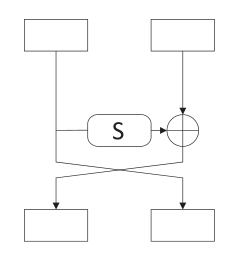
\includegraphics[width=1\linewidth]{feistel.png} }
\caption{Сеть Фейстеля}
\label{fig:image1}
\end{minipage}
\hfill
\begin{minipage}[h]{0.49\linewidth}
\center{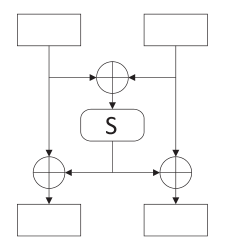
\includegraphics[width=1\linewidth]{laimassey.png} }
\caption{Схема Лая--Месси}
\label{fig:image2}
\end{minipage}
\end{figure}

\newpage
Вставка одиночного рисунка в центре: 

\begin{figure}[h]
\center{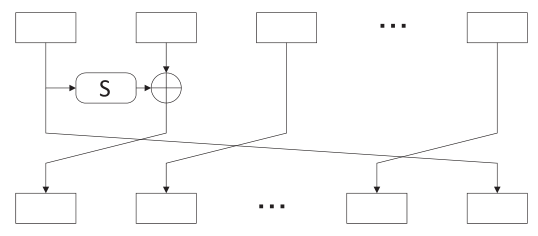
\includegraphics{gfn1.png}}
\caption{Еще схема}
\label{fig:pic3}
\end{figure}

В таблице~\ref{table:cryptosystem} приведены...

\begin{table}[h]
\centering
\begin{tabular}{|c|c|}
\hline
RSA & параметры 1\\
\hline
Classic McEliece & параметры 2\\
\hline
\end{tabular}
\caption{Параметры криптосистемы}
\label{table:cryptosystem}
\end{table}